\section{Basic Memory Layout Considerations}
\label{chap:memory-layout}

\subsubsection*{Element Reference}

In many situations, it is necessary to refer to a specific element in the mesh (for example, to delete a specific face or to query the neighbors of a specific vertex).
There are mainly two ways to realize an \emph{element reference}: pointers or IDs/indices.
As discussed in chapter~2, it is desirable to use growing arrays to store mesh data, making pointers impossible (or at least very difficult) to use as element references.
As a consequence, \code{lox} uses the index of an element in its array to refer to that element.
(Also refer to \cite{sieger2011design} for a discussion about array vs. linked lists and indices vs. pointers.)

Using simple integers as element references in the library's API is not a good idea, however, since it is very easy to use an integer referring to one element kind (e.\,g. a vertex) in a context where a reference to another element kind (e.\,g. a face) is expected.
To avoid this confusion, multiple distinct types are introduced: \code{VertexHandle}, \code{EdgeHandle} and \code{FaceHandle}.
All of those types consist of a single integer field (called the \emph{handle ID}), making them behave exactly like an integer on machine level -- thus having no runtime overhead.
If one is used in the place of another, a compiler \enquote{type mismatch} error is printed, pointing out the bug immediately.
Additionally, a \code{Handle} trait is defined to abstract over all handle types.

Another benefit of dedicated handle types is that the internal integer type can be changed easily (without changing it across the whole codebase).
The default integer type in \code{lox} is a \code{u32} which is sufficient for most meshes in practice.
However, large meshes with more than $2^{32}$ elements require a wider integer type.
With the already mentioned Cargo features, it is possible to configure \code{lox} to used \code{u64} integers in handles, which is sufficient for all meshes in the foreseeable future.

\vspace{2cm}
\subsubsection*{Deleting Elements in a Growable Array}

A simple growing array cannot replace a linked list in all situations, since the latter allows removing elements anywhere in the list in $\mathcal O(1)$ whereas the former only supports removing elements from the end.
Being able to remove arbitrary elements from a mesh required in many situations, so mesh data structures are expected to support it.

There are two possibilities to remove an element at any position inside an array: (a) shift all elements right of the deleted elements one to the left, and (b) store a \code{deleted} flag for each element which is set to \code{true} once an element is deleted.
Solution (a) has a complexity of $\mathcal O(n)$ per remove-operation, making it too slow for most applications.
However, the real problem is that shifting elements invalidates their indices which are used as element reference.
As a consequence, solution (b) has to be used.

\newpage
A problem of the \code{deleted}-flag approach is that elements are not actually deleted but linger in memory, potentially until the whole data structure is freed.
To avoid wasting a lot of memory, programmers should avoid repeatedly adding and removing a large number of elements.
Additionally, the mesh data structure can offer the programmer a way to trigger an internal garbage collection which actually removes deleted elements by reordering the elements in the array.

There are different ways to implement the \code{deleted} flag.
The easiest and most obvious solution in Rust would be to use \code{Vec<Option<T>>} instead of \code{Vec<T>}.
In practice, storing many \code{Option<T>} instances is only a good idea if \code{Option<T>} can use \emph{null value optimization}.
This is usually not the case in the context of mesh data structures, meaning that \code{Option<T>} is notably larger than \code{T}.
Specifically, it is \code{align_of::<T>()} larger, which for structs storing \code{u32} indices is usually 4 bytes.

\begin{figure}[t]
  \centering
  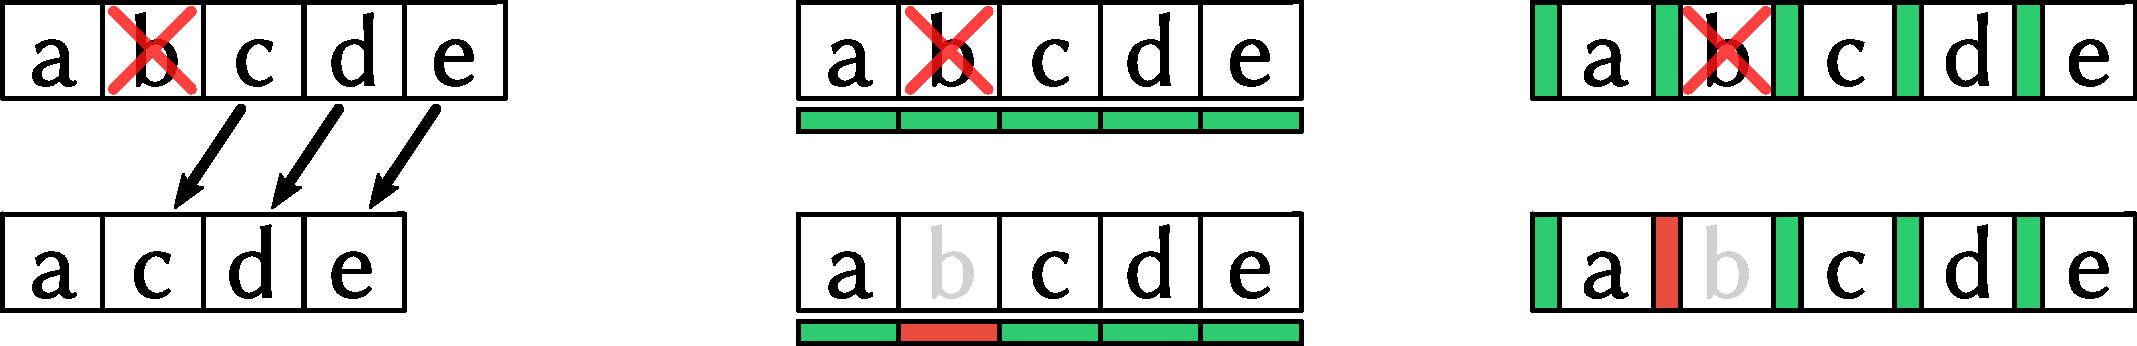
\includegraphics[width=.9\textwidth]{svg2pdf/stable-vec}
  \caption{Different ways to delete an element from a growable array: shifting elements (left), storing a \codebox{deleted} flag as a separate bit-vector (center) and storing a \codebox{deleted} flag next to the elements (right).}
  \vspace{5mm}
\end{figure}

A popular alternative way to store \code{deleted} flags is using a bit-vector, a densely packed array of bits (storing 8 bits per byte).
It has the disadvantage of requiring a separate allocation which slightly increases the reallocation cost and could potentially double the number of cache misses per element access.
However, this is usually out-weight by the benefits:
the dense packing means that no memory is wasted and that many of these flags fit into the cache at once.
For example, a standard-sized L1 cache with 256~KB of storage can fit over 2~million bits, a 64~byte cache line can fit 512 bits.

It is also possible to use special \emph{sentinel values} to mark an element as deleted (this is the general case of null-value optimization, where the sentinel value is 0) or to interleave the bits with the actual values in blocks to avoid an additional allocation.
A proper analysis of these different storage methods would be appropriate, but was outside the scope of this thesis.
In a quick comparison of the \code{Vec<Option<T>>} and bit-vector versions, no large difference in performance was found.
As a consequence and for memory efficiency, the bit-vector implementation was chosen for \code{lox}.
This choice is not final, however, and the implementation could easily be replaced by another one.

The logic for growable arrays that allow deletions is implemented completely independently of \code{lox} in a library called \code{stable-vec}\footnote{\url{https://crates.io/crates/stable-vec}}.
This library is technically also not part of this thesis.





\newpage
\subsubsection*{Property Maps}

As mentioned in chapter 2, it is often necessary to associated arbitrary data with specific mesh elements.
This data is called \enquote{property} in this thesis; vertex normals are a \enquote{vertex property}, for example.
While some properties live as long as the mesh itself (e.\,g. vertex positions or face colors),  others are temporary values that only live for the duration of one algorithm (e.\,g. a Boolean \code{visited} flag).
These temporary properties should not be kept in memory longer than necessary, meaning that they cannot be stored together with the actual elements.
Instead, \code{lox} uses external maps (mapping from element to property), called \emph{property maps}.

These maps can be implemented in a variety of ways, including:

\begin{itemize}
\item A growing array using the handle ID as index (this works because it is already used as an array index in the main mesh).
\item A hash map using the handle ID as key.
\item A list of \code{(handle, value)} pairs.
\end{itemize}

In most situations, the growing array is the best choice as it is very memory efficient and accessing values is very cheap.
However, in a few situations it is necessary to associate values with only a couple of elements.
Using a growing array for that purpose is not a good idea, since the length of the array does not depend on the number of values but on the highest handle ID.
So on average, a growing array would waste a lot of memory, making other implementations a viable choice.

Just like with the mesh data structure, it does not make sense to decide on one specific implementation of external maps.
Instead, all implementations are offered by \code{lox} and abstracted over via traits.
That way, the most fitting implementation can be chosen in every situation.
The corresponding types are currently called \code{VecMap} (growable array), \code{HashMap} and \code{TinyMap} (list of tuples).
The abstraction is realized with three traits to make it as flexible as possible:

\begin{description}
  \item [\codebox{PropMap}] This trait only requires a single method to be implemented.
  Its signature is \code{fn get(&self, handle: H) -> Option<Value>} where \code{H} is the handle type parameter (this is a simplified version of the actual signature, which is explained in chapter~6).
  Returning \code{None} means that no value is associated with the given handle/element.
  This trait represents a simple map from handle to optional value.
  \item [\codebox{PropStore}] Like \code{PropMap}, but can additionally iterate over all handles and values.
  \item [\codebox{PropStoreMut}] Like \code{PropStore}, but can additionally change, insert and remove values.
\end{description}

The three data structures mentioned above (growing array, hash map, list of pairs) implement all three traits.
By using three traits instead of a single one, more exotic types can be used with that interface, too.
The following types are provided by \code{lox} and implement \code{PropMap}, but not the other traits:

\newpage
\begin{itemize}
\item \code{EmptyMap}: contains no properties, always returns \code{None}.
\item \code{ConstMap}: stores a single value and returns that value for all elements/handles.
\item \code{FnMap}: stores a function object with the signature \code{(&self, H) -> Option<Value>} which is used to implement \code{PropMap}.
\end{itemize}

While these types might not seem particularly useful at first, they are immensely handy in some situations.
Of course, they can be replaced by simply preparing a growable array or hash map with the desired values.
This, however, costs memory and extra time.
Specifically, \code{FnMap} is very useful to generate properties without using memory.

As a motivating example, consider an algorithm that produces a float value for each face, thus returning \code{VecMap<FaceHandle, f32>}.
This float value needs to be visualized via colors, for example by simply mapping the float value to gray-scale colors.
With \code{FnMap} a face~$\rightarrow$~color mapping can be created easily without allocating any memory:

\begin{center}
  \begin{minipage}{.59\textwidth}
    \begin{rustcode}
      let face_values = algorithm(&mesh);
      let face_colors = FnMap(|fh| {
          face_values.get(fh).map(to_color)
      });
    \end{rustcode}
  \end{minipage}
\end{center}
\vspace{1cm}

An alternative to external maps is managing all properties in the main mesh type, which is done in OpenMesh and PMP.
Their mesh type has methods like \code{add_face_property} which creates an additional property map managed by that mesh.
Having all mesh data in one object is certainly convenient in many situations, but has disadvantages, too:
it adds a bit of overhead for managing maps dynamically and it is less flexible than having each map as a separate variable.
For these reasons, \code{lox} uses \emph{external} maps.
Users can still create their own struct type with property maps as fields to store all mesh properties in a single type.


\newpage
\subsubsection*{\enquote{Array of Structs} vs. \enquote{Struct of Arrays}}

Having property maps to store mesh properties externally brings up an interesting consideration: is it faster to use one property map per property kind or to use as few different maps as possible (e.\,g. by clustering different property kinds).
This problem is very similar to the \enquote{Array of Structs} (\emph{AoS}) vs. \enquote{Struct of Arrays} (\emph{SoA}) choice.
The two different layout strategies are visualized in figure~\ref{fig:mem-layout-visualization}.

Both layouts use almost the same amount of memory and do not differ in capabilities.
The only difference is in how they interact with CPU caches.
To find an answer to what strategy should be preferred, a number of different benchmarks were conducted.

\begin{figure}[t]
  \centering
  \newcommand{\pointerbox}{%
    \parbox{1.2cm}{%
      \tikz{%
        \draw (-3.2mm,-3.2mm) rectangle (3.2mm,3.2mm);
        \draw[line width=.4mm, {Circle[length=1.5mm,width=1.5mm]}-{Triangle[length=2.2mm,width=2.7mm]}](-0.75mm,0)--(1.2cm,0);
      }%
    }
    \hspace{2mm}
  }
  \renewcommand{\arraystretch}{1.1}
  \setlength{\dashlinedash}{.4mm}
  \setlength{\dashlinegap}{.4mm}

  \begin{subfigure}[b]{.55\textwidth}
    \centering
    \setlength{\tabcolsep}{0mm}
    \pointerbox
    \begin{tabular}{|C{6.2mm}:C{6.2mm}:C{6.2mm}|C{6.2mm}:C{6.2mm}:C{6.2mm}|C{6.2mm}:C{6.2mm}:C{6.2mm}|}\hline
      $a_0$ & $b_0$ & $c_0$ & $a_1$ & $b_1$ & $c_1$ & $a_2$ & $b_2$ & $c_2$ \\\hline
    \end{tabular}
    \vspace{7mm}
    \caption{Array of Structs.}
  \end{subfigure}%
  %
  \begin{subfigure}[b]{.35\textwidth}
    \centering
    \setlength{\tabcolsep}{0mm}
    \pointerbox
    \begin{tabular}{|C{6.2mm}|C{6.2mm}|C{6.2mm}|}\hline
      $a_0$ & $a_1$ & $a_2$ \\\hline
    \end{tabular}\\[-.5mm]
    \pointerbox
    \begin{tabular}{|C{6.2mm}|C{6.2mm}|C{6.2mm}|}\hline
      $b_0$ & $b_1$ & $b_2$ \\\hline
    \end{tabular}\\[-.5mm]
    \pointerbox
    \begin{tabular}{|C{6.2mm}|C{6.2mm}|C{6.2mm}|}\hline
      $c_0$ & $c_1$ & $c_2$ \\\hline
    \end{tabular}
    \caption{Struct of Arrays.}
  \end{subfigure}

  \renewcommand{\arraystretch}{1.0}

  \caption{The two different memory layouts (three items with three fields each).}
  \label{fig:mem-layout-visualization}
\end{figure}

In these benchmarks, many items with a few random \code{u32} fields were stored in either one of the two memory layouts.
The time required to sum up all or some of these values was measured to get an idea of the respective speeds.
The different benchmarks attempted to cover the following parameter space:

\begin{itemize}
  \item \textbf{Memory layout}: AoS or SoA.
  \item \textbf{Traversal kind}: random or sequential.
  In the sequential benchmarks, a loop simply iterates sequentially over all indices starting from 0.
  The random benchmarks use the first field's \code{u32} value as next index to jump to.
  This was done to not include the generation of random numbers in the measured time.
  Notably, these \code{u32} values were already generated to be valid indices (i.\,e. smaller than the total number of items) and thus, the timed code does not need to perform any additional work on these values.
  \item \textbf{Total number of items}: all benchmarks were performed with 10,000, 100,000, 1,000,000 and 10,000,000 items.
  \item \textbf{Number of [used] fields per item}: 1:1, 2:1, 2:2, 4:1, 4:2, 4:4, 6:1, 6:3 and 6:6 were tested.
  The syntax X:Y means that each item has X many fields and Y many fields were included in the sum, the other fields were ignored.
\end{itemize}

\vfill

Getting reliable data from a benchmark is difficult because many factors need to be considered -- failing to pay attention to one of them could render the measured data useless.
To deal with the inherent noise, almost all benchmarks execute the code that needs to be measured many times and analyze all measured durations to obtain a useful point estimate (e.\,g. the mean).
Performing a benchmark that attempts to measure the effect of CPU caches is particularly challenging, because the cache state persists over multiple iterations of the same code.
That in turn means that repeated measurements are not independent of one another, making the measured data unusable or very hard to analyze.

\newpage
One idea on how to tackle this problem is to simply flush all caches.
This is actually possible on most x86-64 CPUs with the \code{WBINVD} instruction, which first writes all cache contents back to main memory and then invalidates all CPU internal caches\footnote{There is also the \codebox{INVD} instruction which invalidates caches without writing them back, but it is highly unsafe as it globally destroys the consistency of memory operations, likely crashing or corrupting all programs currently running on the CPU (including the kernel).}.
As \code{WBINVD} is a privileged instruction, it can only be executed in ring 0 (the kernel mode).
But since benchmarks should not run in kernel mode, a special kernel module was loaded, allowing user-land programs to trigger execution of \code{WBINVD}.
The benchmarking code would use that trigger before each repetition of the benchmarked code.

Unfortunately, executing the instruction via the kernel module itself takes a significant amount of time (approximately 750\,µs on the benchmark machine).
Many of the benchmarks have a per-iteration time of less than that, making \code{WBINVD} a non-tolerable overhead.
Excluding the duration of cache invalidation from the total measured time is not easily possible either.
Since measuring short durations does not yield reliable data, multiple repetitions are measured together and not on their own.
Because of this massive overhead, \code{WBINVD} was dropped as possible solution.

Instead, each repetition of the benchmark was performed on separate data.
Before executing the benchmarked code, a copy of the working data was prepared for each iteration, meaning that the cache state produced by one repetition does not affect other iterations.
As CPU caches have very complex behavior, the absence of cross-repetition cache effects cannot be completely guaranteed, but the probability of them occurring was reduced substantially.

The benchmark code and more details on the benchmark can be found in the repository of this thesis in the folder \code{benchmarks/memory-layout/}.
The benchmark uses the framework \emph{Criterion} \cite{criterion} which features a sophisticated statistical analysis of the raw measurements.
However, only the mean and standard deviation were used to produce the graph seen in this report.

The full benchmark ran for approximately three hours and was performed on a completely idle \textsf{Thinkpad T-460p}, containing an \textsf{Intel i7-6700\,HQ} and running \textsf{Ubuntu 18.04}.
The \textsf{Intel i7-6700\,HQ} has 6\,MiB of L3 cache, 1\,MiB of L2 cache and 256\,KiB of L1 cache.
Figure~\ref{fig:memory-layout-bench} shows the benchmark results, which are discussed on the page thereafter.

\begin{figure}[p]
  \centering
  \vspace{-7mm}
  \centerline{
    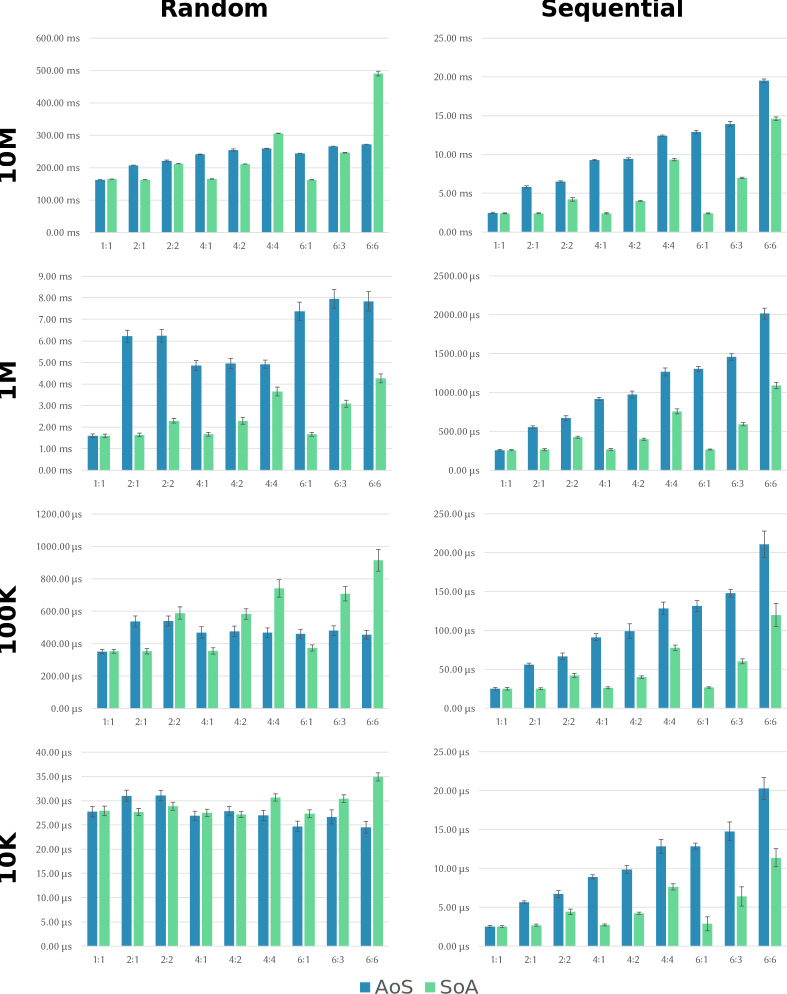
\includegraphics[width=1.18\textwidth]{svg2pdf/SOAvsAOS}
  }
  \caption{
    Results of the memory layout benchmark.
    The numbers on the far left show the total number of items.
    The label for each pair of bars encodes the number of fields: \textsf{X:Y} means that each item has \textsf{X} fields, \textsf{Y} of which are used.
    The height of the bars is the mean of all measurements, the error bar displays the standard deviation.
  }
  \label{fig:memory-layout-bench}
\end{figure}

\newpage

The results of the benchmark allow various interesting observations:

\begin{itemize}
  \item The type of traversal plays a massive role in performance: in the 10M items benchmarks, random traversal is approximately 50 to 70 times slower than the sequential traversal.
  The difference is a bit smaller for the benchmark with fewer items, but still substantially.
  This effect is very much expected.
  \item The durations for sequential traversal scale pretty closely with the number of items.
  This is to be expected, because in those benchmarks, any caching effects should be very small and all other operations should scale linearly.
  On the other hand, the durations for random traversal do \emph{not} scale linearly with number of items, due to non-linear cache effects.
  The difference between 1M and 10M items is particularly high.
  \item The durations of \textsf{1:1} benchmarks do not differ between memory layouts, which is expected: for one field, the memory layouts are the same.
  This is a confirmation that there are no unexpected differences in the benchmarks of different memory layouts.
  \item The duration for SoA benchmarks does not depend on the total number of fields, but just on the number of \emph{used} fields.
  For example, \textsf{1:1}, \textsf{2:1}, \textsf{4:1} and \textsf{6:1} take the same time.
  This makes sense because adding additional, unused fields does not affect which memory is accessed by the SoA benchmark.
  \item For random traversal with 10K, 100K or 1M items in AoS layout, the benchmarks with two total fields take longer than the benchmarks with four (and sometimes six) total fields.
  This is not expected and could thus point to a flaw in the benchmark.
  The benchmark was checked again, but no reasons for this behavior could be found.
\end{itemize}

Comparing the two memory layouts, one important first observation is that SoA always outperforms AoS for sequential traversal, especially so for benchmarks where not all fields are used.
The latter is expected: when loading one cache line, it only contains values that are actually used in the SoA case.
In the AoS case however, the cache line also contains unused fields.
As a consequence, if some fields are unused, SoA requires fewer cache lines to be loaded from main memory compared to AoS.


The comparison becomes more complicated for random traversal.
In general, the expected behavior is that AoS causes one cache miss per item, while SoA causes one cache miss per field.
This would mean that AoS should outperform SoA for multiple fields.
This is not always the case, however.
For 10K items, both memory layouts perform mostly equally well.
With 100K items, SoA outperforms AoS if only one field is used, but is up to two times slower than AoS if two or more fields are used.
The benchmarks where SoA is faster can be explained by the denser packing of the one used field: all cache lines contain only useful data, increasing the number of items fitting into the cache which in turn increases the chance of finding a random item in the cache.

Completely unexpectedly, for 1M items, SoA significantly outperforms AoS in all benchmarks.
Something that might explain this behavior is the size of the test CPU's L3 cache (6\,MiB) compared to the total size of test data:
one million items with \code{u32} fields corresponds to 4\,MiB (one field) to 24\,MiB (six fields) of data.
In the \textsf{1:1} case, all data fits into the L3 cache, meaning that on average, the main memory only needs to be accessed $4 \text{\,MiB} / 64 \text{ Bytes (the size of one cache line)} = 65,536$ times.
For more fields, the full data does not fit into the L3 cache, meaning that some cache lines might need to be loaded multiple times from main memory.
The difference between memory layouts \emph{might} be due the specific associativity and replacement strategy of the L3 cache.

For 10M items, SoA slightly outperforms AoS for one or two used fields, but is slightly slower for four used fields and twice as slow for six used fields.
Due to the total size of the data (40\,MiB to 240\,MiB), the probability to find a value in the L3 cache is very low: between 15\% and 2.5\%.
Hence, most memory reads actually need to access main memory.
The rather small difference in duration between one and two used fields for the SoA layout can be explained by CPU pipelining: two memory operations can potentially be executed in parallel, meaning that the wait time for both accesses overlap.

\vspace{1.5cm}

In summary, neither memory layout is superior in all situations.
While many memory access patterns for mesh operations (e.\,g. depth first search) tend to have a very random nature, iterating sequentially over all elements of a mesh is not uncommon either.
Thus, benchmarks of both traversal kinds are important to consider.
Analyzing this benchmark lead to the following consequences for the development of \code{lox}:

\begin{itemize}
  \item Using multiple external property maps is usually fine.
  For that reason, \code{lox} does not yet allow storing mesh properties next to adjacency information, i.\,e. a \code{HalfEdgeMesh} cannot store vertex positions.
  This feature might be added in the future, though.
  \item If an algorithm defines multiple mesh properties that are always used together, it is often preferred to cluster them into one property map.
  \item Generally, the more convenient solution can be used.
  To improve performance of a specific algorithm, that algorithm should be benchmarked with both memory layouts, as these specific benchmarks are often more useful than highly artificial ones, like this one.
\end{itemize}
